\documentclass[conference]{IEEEtran}

\usepackage{graphicx}
\usepackage{float}
\usepackage{easy-todo}
\usepackage{tabularx}
\usepackage{array}
\usepackage[hidelinks]{hyperref}
\usepackage{algorithm}
\usepackage{algpseudocode}
\usepackage{placeins}
\usepackage{stfloats}

\algrenewcommand\algorithmiccomment[1]{\hfill$\triangleright$ #1}

\begin{document}

\title{Experimental Evaluation and Optimization of
  Real-Time Scheduling on STM32}
\author{
	\IEEEauthorblockN{Vladimir Toporkov, Artem Burmyakov}
	\IEEEauthorblockA{
		\textit{Innopolis University}
	}
}
\maketitle

\section{Introduction}
\subsection{Contribution}

Our contributions are about evaluation of schedulers for STM32 microcontroller:
%
\begin{itemize}
\item we first implement Super Loop scheduler,
\item then we implement the Earliest-Deadline First (EDF) scheduler, and finally
\item we evaluate their performance upon a real STM32 hardware.
\end{itemize}

\section{Background on STM32}

The experimental platform consists of a uniprocessor STM32F767 microcontroller and external sensors connected through its hardware peripherals, as shown in Fig.~\ref{fig:stm32_hw}.

\begin{figure}[htbp]
  \centering
  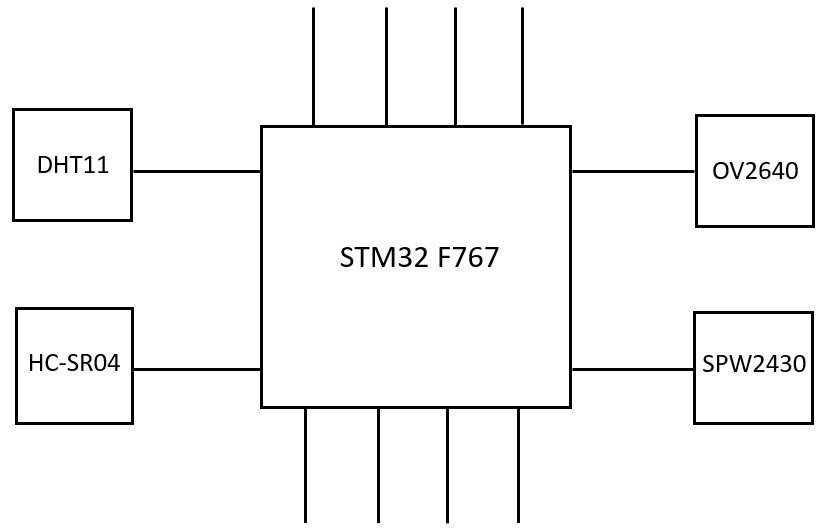
\includegraphics[width=0.9\columnwidth]{stm32_hardware_platform.png}
  \caption{STM32 hardware platform and connected sensors.}
  \label{fig:stm32_hw}
\end{figure}

The hardware components are presented in Table~\ref{tab:hardware}.

\begin{table}[H]
	\centering
	\caption{Experimental hardware platform.}
	\label{tab:hardware}
	
	\small
	\renewcommand{\arraystretch}{1.15}
	\setlength{\tabcolsep}{6pt}
	
	\begin{tabularx}{\columnwidth}{l>{\centering\arraybackslash}X}
		\hline
		\textbf{Component} &
		\textbf{Purpose} \\
		\hline
		
		STM32F767 &
		Scheduling and task execution \\
		
		DHT11 &
		Temperature and humidity measurement \\
		
		HC-SR04 &
		Distance measurement \\
		
		OV2640 &
		Image capturing \\
		
		SPW2430 & 
		Acoustic signal acquisition \\
		
		\hline
	\end{tabularx}
\end{table}

\section{System Model}
\label{sec:system_model}

We model the workload by a set of periodic tasks $\mathcal{T}=\{\tau_1,\ldots,\tau_n\}$ executed on a uniprocessor. We consider only implicit deadlines, i.e, $D_i=T_i$. Each task $\tau_i=(C_i,T_i=D_i)$ generates a sequence of jobs $J_i^j$, where $j$ denotes the scheduled release index. Consecutive scheduled releases satisfy $R_i^{j+1}=R_i^j+T_i$.

\begin{table}[htbp]
  \centering
  \caption{System model notation.}
  \label{tab:system_model}
  \small
  \renewcommand{\arraystretch}{1.15}
  \begin{tabularx}{\columnwidth}{l >{\raggedright\arraybackslash}X}
    \hline
    \textbf{Symbol} & \textbf{Meaning} \\
    \hline
    $\mathcal{T}, n$ & Task set and number of tasks \\
    $\tau_i$ & Task $i$ \\
    $C_i$ & Execution time of a job of $\tau_i$ \\
    $T_i$ & Task period \\
    $D_i=T_i$ & Relative deadline, equal to the period \\
    $J_i^j$ & Job associated with the $j$-th scheduled release of $\tau_i$ \\
    $R_i^j$ & Scheduled release time \\
    $f_i^j$ & Completion time of an executed job \\
    $d_i^j=R_i^j+D_i$ & Absolute deadline \\
    $U=\sum_{i=1}^{n} C_i/T_i$ & Task-set utilization \\
    \hline
  \end{tabularx}
\end{table}

Table~\ref{tab:system_model} summarizes the notation. Release indices include skipped activations, for which no completion time is defined.

\begin{itemize}
  \item A schedule specifies which job executes on the processor at each time instant, or whether the processor executes no job.
  \item Preemption interrupts a job before completion to execute another job. The interrupted job may resume later.
  \item A completed job $J_i^j$ has missed its deadline if $f_i^j>d_i^j$.
\end{itemize}

\section{Scheduling Principles}
\label{sec:sched_principles}

\subsection{Super Loop Scheduler}
The considered Super Loop scheduler repeatedly scans tasks in a fixed order and executes each selected job non-preemptively. To illustrate its behavior, let us consider the two periodic tasks in Table~\ref{tab:superloop_tasks}. Both tasks first release at $t=0$.

\begin{table}[H]
  \centering
  \caption{Task set used in the Super Loop example.}
  \label{tab:superloop_tasks}
  \begin{tabular}{c|ccc}
    \hline
    \textbf{Task} & $C_i$ & $T_i$ & $D_i$ \\
    \hline
    $\tau_1$ & 20 & 50 & 50 \\
    $\tau_2$ & 10 & 20 & 20 \\
    \hline
  \end{tabular}
\end{table}

The resulting Super Loop schedule is shown in Fig.~\ref{fig:superloop_schedule}.

\begin{figure*}[tb]
  \centering
  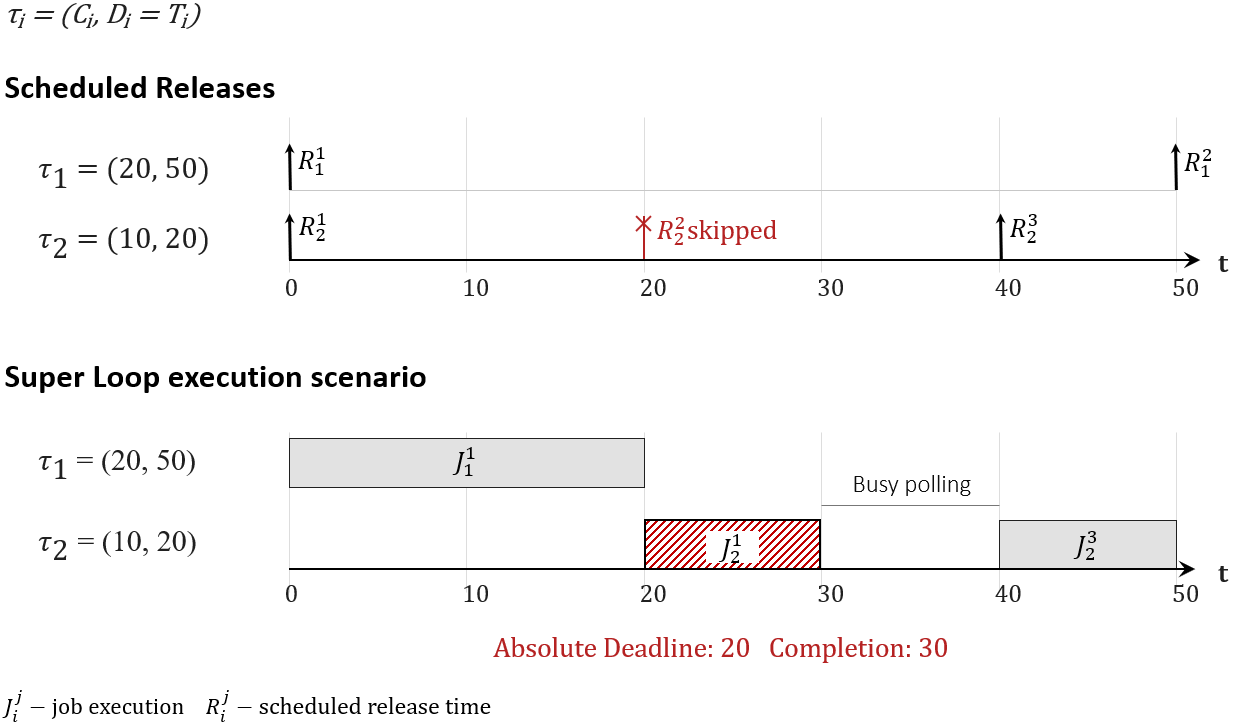
\includegraphics[width=0.9\textwidth]{superloop_execution_schedule.png}
  \caption{Super Loop execution scenario for the task set in Table~\ref{tab:superloop_tasks}.}
  \label{fig:superloop_schedule}
\end{figure*}

Let $t^{cur}$ denote the current system time and $t_i^{next}$ the next scheduled release time of task $\tau_i$. During execution of $J_i^j$, the release variable $t_i^{next}$ retains $R_i^j$. At completion, $f_i^j$ denotes the completion time, and a deadline miss is recorded if $f_i^j>d_i^j$. The scheduler then advances $t_i^{next}$ by $T_i$. While $t_i^{next}<f_i^j$, the scheduled release at $t_i^{next}$ is counted as skipped and $t_i^{next}$ is advanced by $T_i$ again. A release at $t_i^{next}=f_i^j$ is retained.

Algorithm~\ref{alg:superloop} summarizes the illustrated scheduling logic. Since $R_i^1=0$, the release index is $j=1+t_i^{next}/T_i$, including skipped releases. The clock used by \textsc{Now} starts at zero.

The corresponding scheduling state is shown in Table~\ref{tab:superloop_state}.

\begin{table}[H]
  \centering
  \caption{Super Loop scheduling state for Fig.~\ref{fig:superloop_schedule}.}
  \label{tab:superloop_state}

  \small
  \renewcommand{\arraystretch}{1.2}
  \setlength{\tabcolsep}{3pt}

  \begin{tabularx}{\columnwidth}{
    c c c
    >{\centering\arraybackslash}X
    >{\centering\arraybackslash}X}
    \hline
    $t^{cur}$ &
    $t_1^{next}$ &
    $t_2^{next}$ &
    Deadline miss check &
    Release skip check \\
    \hline

    0 & 0 & 0 &
    -- &
    -- \\

    20 & 50 & 0 &
    $20 < R_1^1 + 50$ &
    $20 < R_1^2$ \\

    30 & 50 & 40 &
    \textbf{$30 > R_2^1 + 20$} &
    \begin{tabular}{c}
      \textbf{$30 > R_2^2$} \\
      $30 < R_2^3$
    \end{tabular} \\

    40 & 50 & 40 &
    -- &
    -- \\

    50 & 50 & 60 &
    $50 < R_2^3 + 20$ &
    $50 < R_2^4$ \\

    \hline
  \end{tabularx}
\end{table}

In Fig.~\ref{fig:superloop_schedule}, $J_1^1$ executes from $t=0$ to $t=20$. Then, $J_2^1$ executes until $t=30$, missing its deadline at $t=20$. At completion, the release scheduled for $R_2^2=20$ is counted as skipped and $t_2^{next}$ advances to $R_2^3=40$. Thus, no $J_2^2$ is executed.

\begin{algorithm}[!t]
	\caption{Super Loop Scheduler}
	\label{alg:superloop}
	\begin{algorithmic}[1]
		
		\Function{SuperLoop}{$\mathcal{T}$}
		
		\ForAll{$\tau_i \in \mathcal{T}$}
		\State $t_i^{next} \gets 0$
		\EndFor
		
		\While{true}
		
		\For{$i \gets 1$ to $n$}
		\Comment{Fixed task order}
		
		\State $t^{cur} \gets \Call{Now}{}$
		
		\If{$t^{cur} \geq t_i^{next}$}
		
		\State $j \gets 1+t_i^{next}/T_i$
		\State $R_i^j \gets t_i^{next}$
		\State \Call{Execute}{$J_i^j$}
		\Comment{Non-preemptive}
		
		\State $f_i^j \gets \Call{Now}{}$
		
		\If{$f_i^j > R_i^j + D_i$}
		\State \Call{RecordMiss}{$J_i^j$}
		\EndIf
		
		\State $t_i^{next} \gets t_i^{next} + T_i$
		
		\While{$t_i^{next} < f_i^j$}
		\State \Call{RecordSkip}{$\tau_i, t_i^{next}$}
		\State $t_i^{next} \gets t_i^{next} + T_i$
		\EndWhile
		
		\EndIf
		
		\EndFor
		
		\EndWhile
		
		\EndFunction
		
	\end{algorithmic}
\end{algorithm}

\subsection{Earliest Deadline First}
Unlike Super Loop, Earliest Deadline First (EDF) selects jobs according to their absolute deadlines.

We first consider preemptive EDF with immediate preemption. At each scheduling decision, the ready job with the earliest absolute deadline $d_i^j$ is selected (Section~\ref{sec:system_model}). If a newly released job has an earlier absolute deadline than the running job, it preempts the running job.

Figure~\ref{fig:edf_schedule} illustrates EDF scheduling for the same task set. Both tasks first release at $t=0$.

\begin{figure*}[!b]
	\centering
	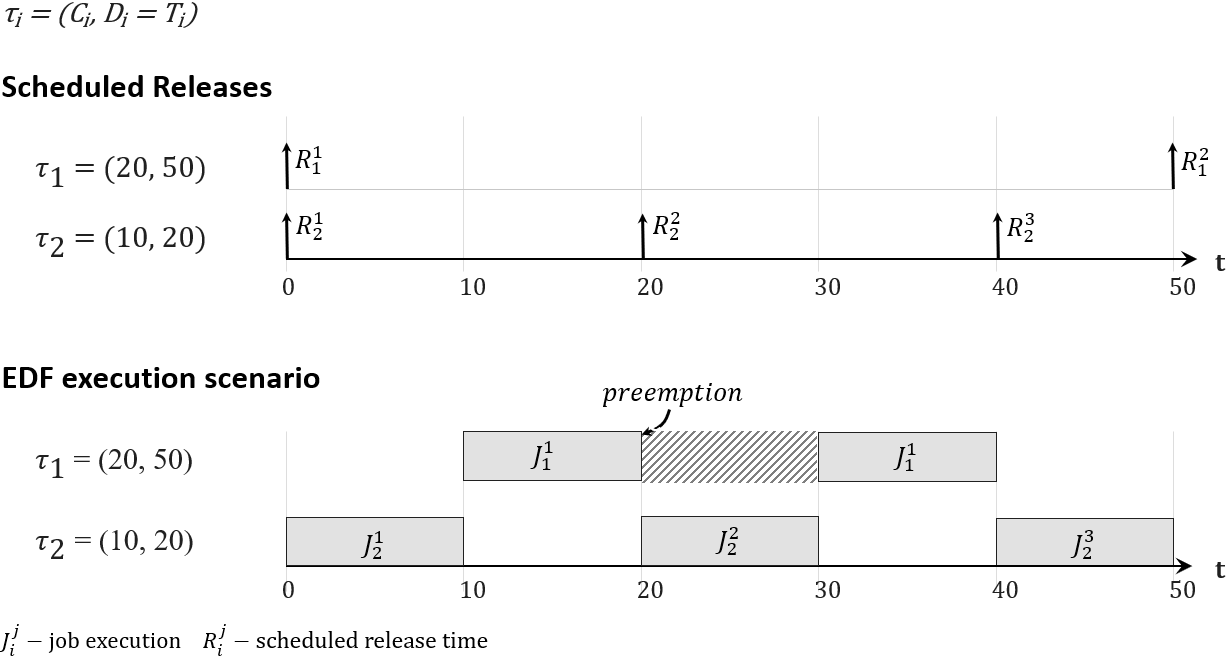
\includegraphics[width=0.9\textwidth]{edf_execution_schedule.png}
	\caption{EDF execution scenario for the task set in Table~\ref{tab:superloop_tasks}. Hatching indicates a preempted
		job awaiting resumption.}
	\label{fig:edf_schedule}
\end{figure*}

At $t=20$, $J_2^2$ is released with $d_2^2=40<d_1^1=50$ and preempts $J_1^1$. After $J_2^2$ completes at $t=30$, $J_1^1$ resumes and completes at $t=40$.

The implementation on STM32 approximates preemption using fixed-size execution chunks. A running job may therefore be preempted only after the current chunk completes. Consequently, an earlier-deadline job can experience a bounded preemption delay.

In Fig.~\ref{fig:chunked_edf}, $J_2^2$ is released while $J_1^1$ is executing its current chunk. Although $J_2^2$ has the earlier absolute deadline, preemption occurs only at the end of the current chunk.

\begin{figure*}[!b]
	\centering
	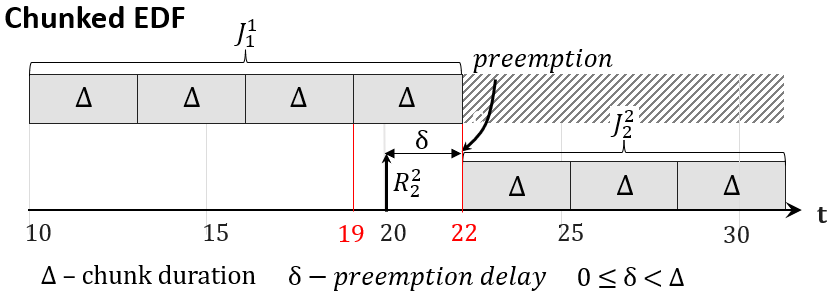
\includegraphics[width=0.8\textwidth]{chunked_edf_execution_schedule.png}
	\caption{Chunk-bounded preemption in the EDF implementation.}
	\label{fig:chunked_edf}
\end{figure*}

In the considered implementation, preemption is deferred until the current execution chunk completes. In Fig.~\ref{fig:chunked_edf}, this results in a preemption delay of $\delta=2$ ms.

\section{Performance Evaluation}
 \begin{figure}[H]
  \centering
  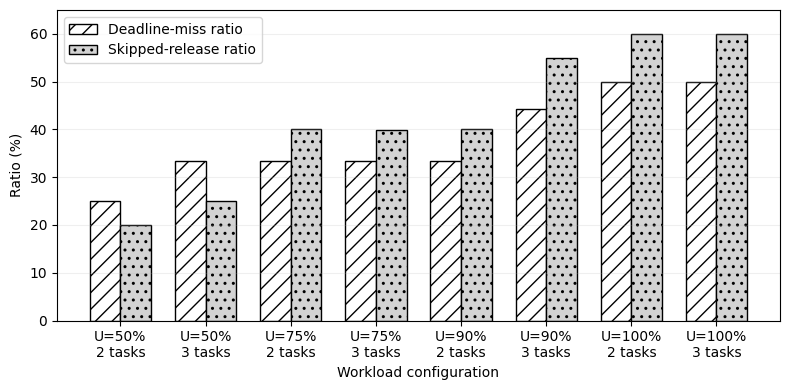
\includegraphics[width=\columnwidth]{superloop_performance_results.png}
  \caption{Per-task deadline-miss and skipped-release ratios under Super Loop. Each configuration specifies the task-set utilization $U$ and the number of tasks.}
  \label{fig:superloop_baseline}
 \end{figure}

\end{document}
